\documentclass{article}
\usepackage[utf8]{inputenc}
\usepackage[T1]{fontenc}
\usepackage[francais]{babel}
\usepackage{lmodern}
\usepackage{graphicx}
\usepackage{geometry}

\geometry{hmargin=30pt, vmargin=30pt}

\title{Bilan mi-parcours : IHM Ecriture sur Tableau Virtuel}
\author{Bollini Kevin, Mélia Geoffrey, Pagès Julien, Saleil Baptiste}
\date{2 Mars 2012}

\begin{document}

\maketitle
	Nom du groupe : \textbf{PouerMouer}
	\section{Composition du groupe et contact}
	
	\begin{itemize}
	\item Kevin Bollini : kevin.bollini@etud.univ-montp2.fr \\
	\item Geoffrey Mélia : geoffrey.melia@etud.univ-montp2.fr \\
	\item Julien Pagès : julien.pages01@etud.univ-montp2.fr \\
	\item Baptiste Saleil : baptiste.saleil@etud.univ-montp2.fr \\
	\end{itemize} 	
	\section{Planning}
		\begin{center}
			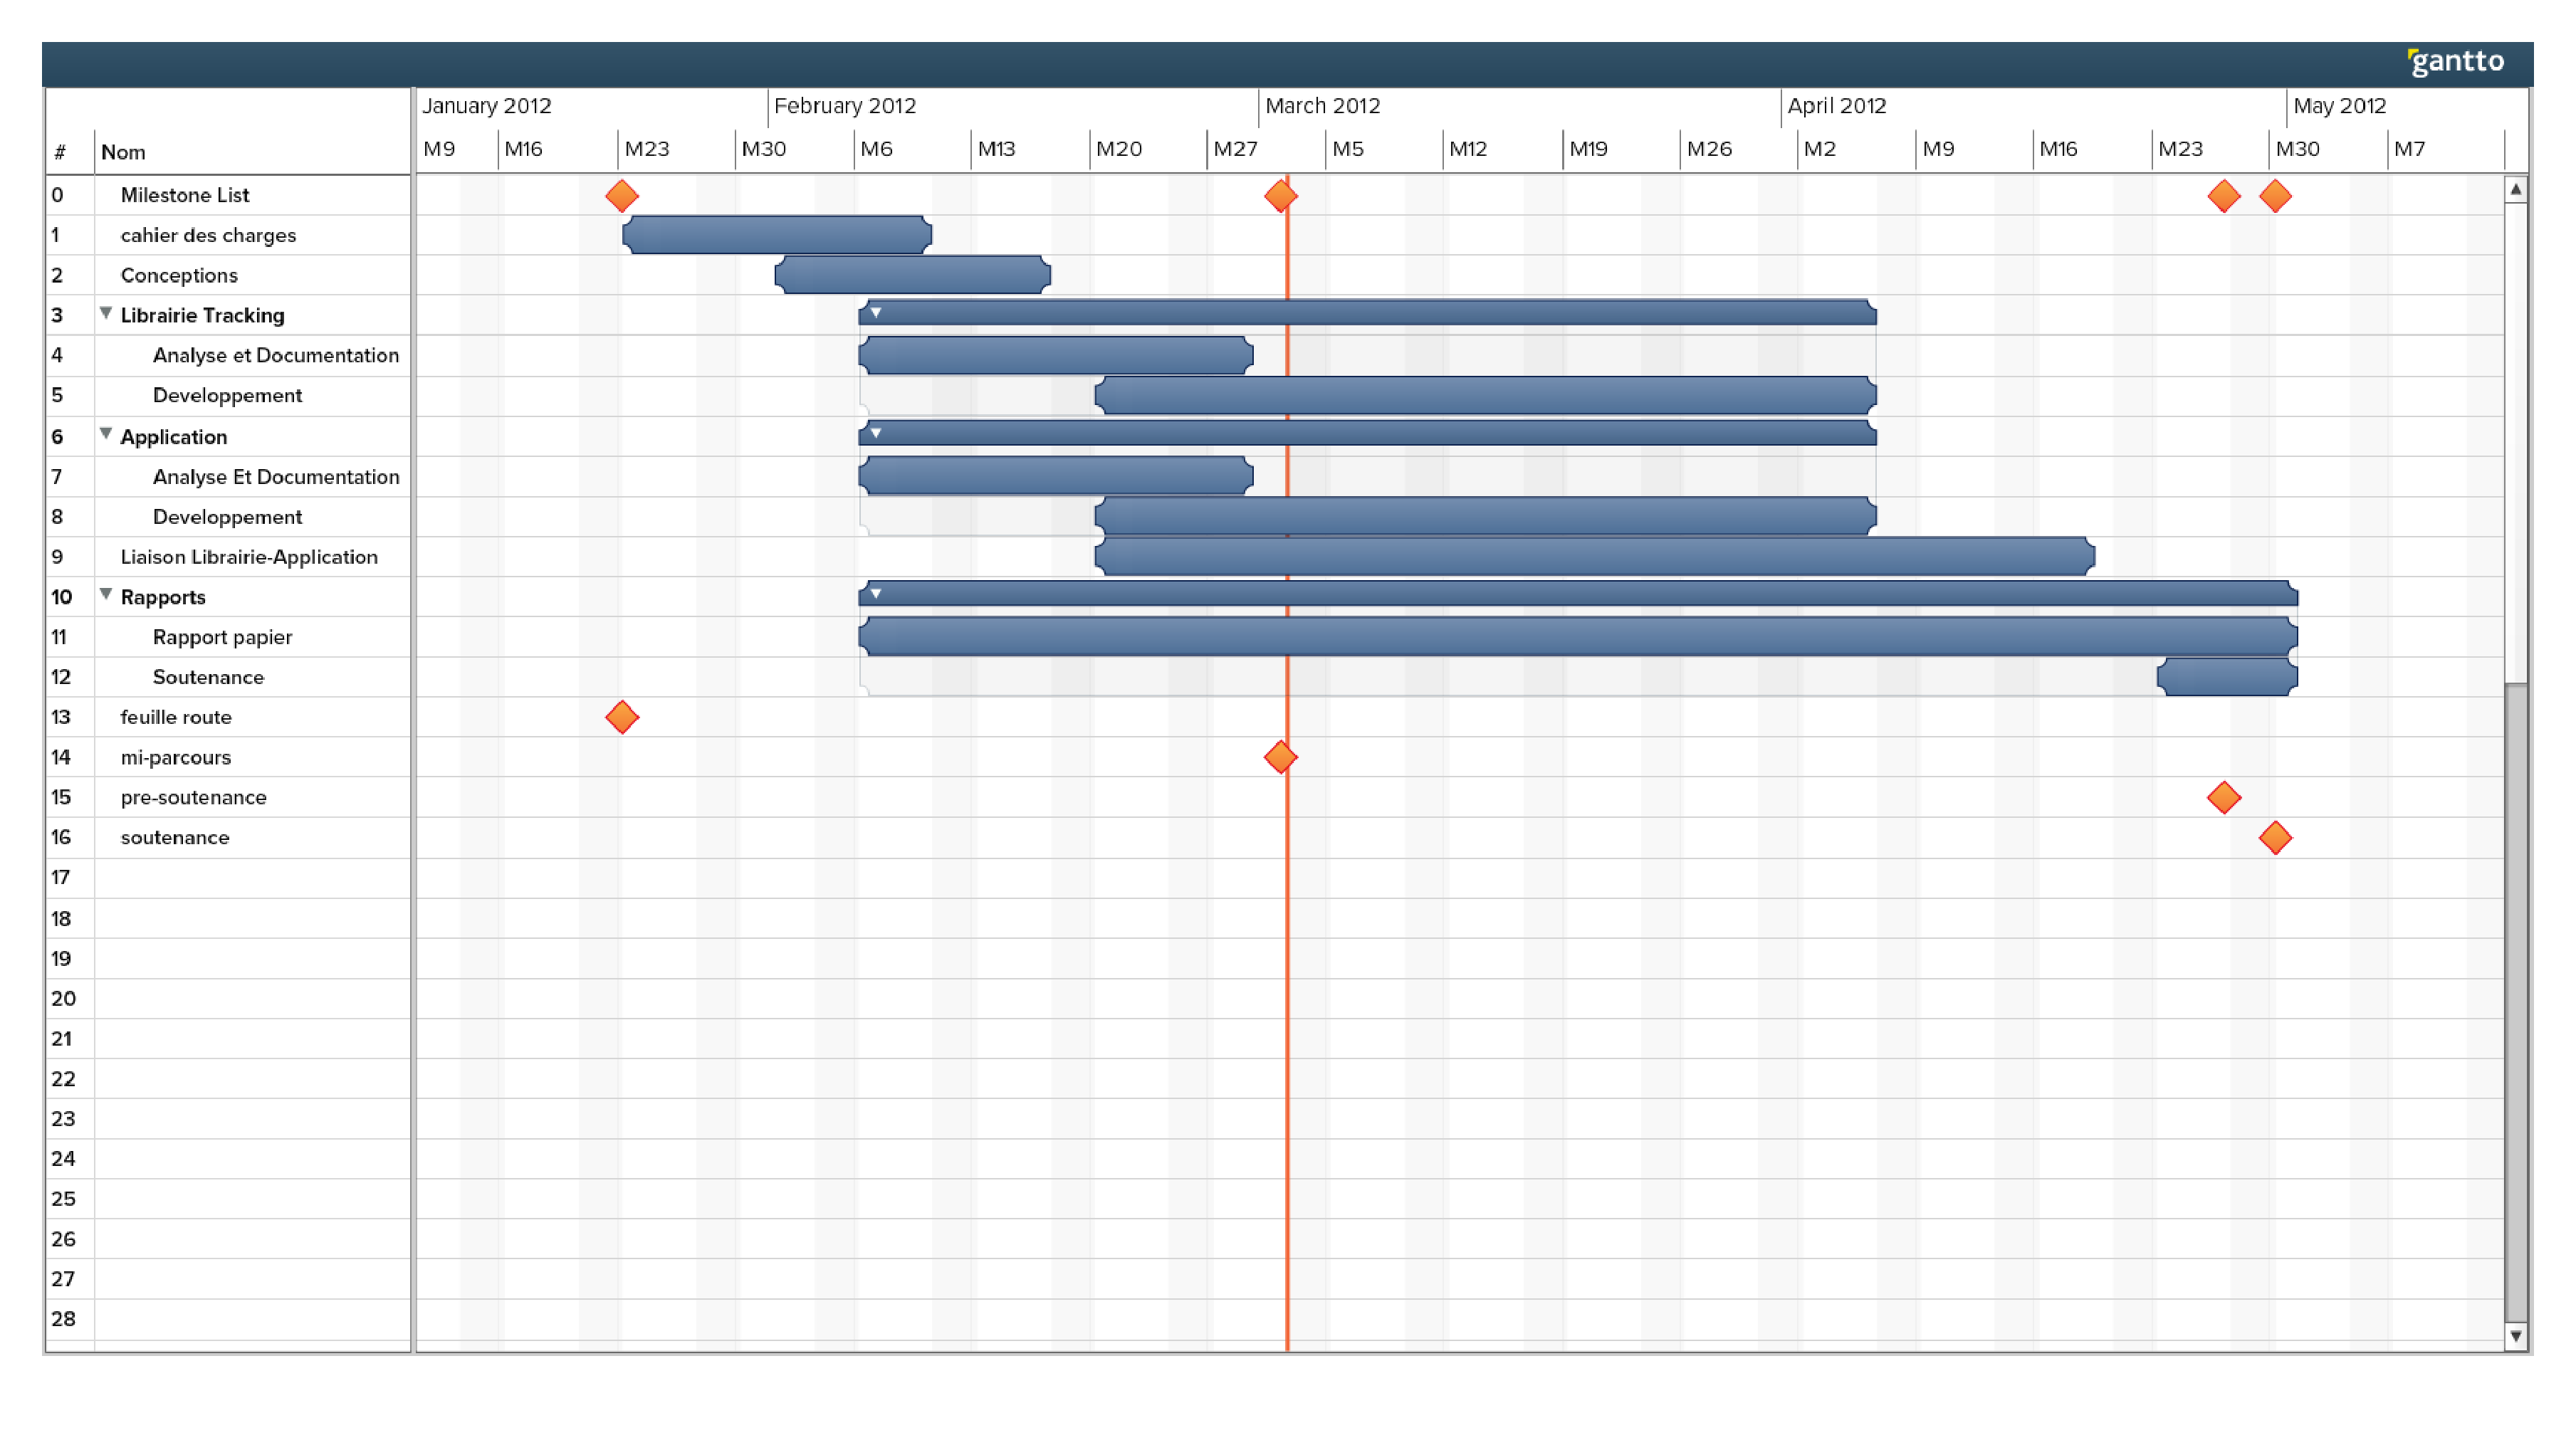
\includegraphics[scale=0.3]{retroplanning.pdf}
			\it rétro-planning, état actuel du projet
		\end{center}
	\section{Tâches effectuées}
		Une première version archaïque de l'application, permettant pour l'instant de réaliser une capture des mouvements d'un objet coloré et de les enregistrer sous forme de nuage de points sur le tableau blanc.
		\subsection{Librairie}
			L'analyse et la conception de la librairie à été réalisée. Une première méthode de track naif par couleur à été implémentée et est utilisée par l'application. D'autre part, une méthode de track par forme est terminée mais n'est pas encore utilisable par l'application.
		\subsection{Logiciel}
	\section{Problèmes rencontrés}
		\subsection{Librairie}
			Passée l'étape de l'analyse, la difficulté majeure que nous avons pour l'instant rencontrée fut la création d'un algorithme de détection des formes tirant parti de la puissance d'OpenCV. Nous avons en effet envisagé plusieurs manières de parvenir à cette recherche de forme : composantes connexes, détection des contours ou encore concordance de templates (comparaison d'images, méthode que nous avons finalement privilégiée).
		\subsection{Logiciel}
			bla
			\paragraph{Note : \\}
				En revanche, grâce à une séparation en deux parties bien distinctes de notre projet et grâce à une rigueur de travail, nous n'avons rencontré aucune difficulté à effectuer la liaison entre la librairie et l'application en elle-même.
	\section{Tâches restantes}
		\subsection{Librairie}
			Mise en place des fonctions d'initialisation de track par forme et optimisation de celles par couleur.\\
			Implémentation d'une méthode de track mélangeant le track par forme et par couleur.\\
		\subsection{Logiciel}
\end{document}

